\section{Refractive index and dispersion}
\label{sec:dispersion}

This section gives a brief overview over the refractive index.

When considering light in the objective of electromagnetic optics we find that the complex refractive index
\begin{equation}
    \underline{n} = n + i \kappa \label{eq:refindex}
\end{equation}
includes the  regular refractive index  $n$ and an imaginary component -- the optical extinction coefficient
 $\kappa$. The refractive index $n$ is related to the 
phase velocity $\nu$ of the electromagnetic wave inside the medium. The extinction coefficient $\kappa$ gives 
in accordance with the Beer-Lambert-Law the rate of exponential decay as can be seen
by considering a plane wave ansatz
\begin{equation}
    \mathbf{E}(s,t) = \mathrm{Re}[ \mathbf{E}_{0} e^{i( \underline{k} x-\omega t)}]  = 
    \mathrm{Re}[ \mathbf{E}_{0} e^{i( \frac{2 \pi (n + i \kappa)}{\lambda_0} x-\omega t)}] =
    e^{\frac{2 \pi \kappa x}{\lambda_0}}\mathrm{Re}[ \mathbf{E}_{0} e^{i( k x-\omega t)}]
\end{equation}
using the complex wave number $\underline{k} = \frac{2 \pi (\underline{n})}{\lambda_0}$. The refractive index $n$
and the optical extinction coefficient can be linked using the Kramers-Kronig relations as those two numbers can be 
derived from the complex susceptibility $\underline{\chi}$.

As an example we derived the refractive index $n$ using the Kramers-Kronig relations from $\kappa$ for Germanium. For this we made the
approximation of low absorption. Therefore 
\begin{gather*}
    \kappa \approx - \mathrm{Im}[\underline{\chi}]\\
    \mathrm{and}\\
    n \approx \sqrt{1 + \mathrm{Re}[\underline{\chi}]}
\end{gather*}
are assumed to be true. Afterwards the calculation is compared to the real data. This shows that knowing one quantity, we can derive the other using the Kramers-Kronig relations.

\begin{figure}
    \centering
    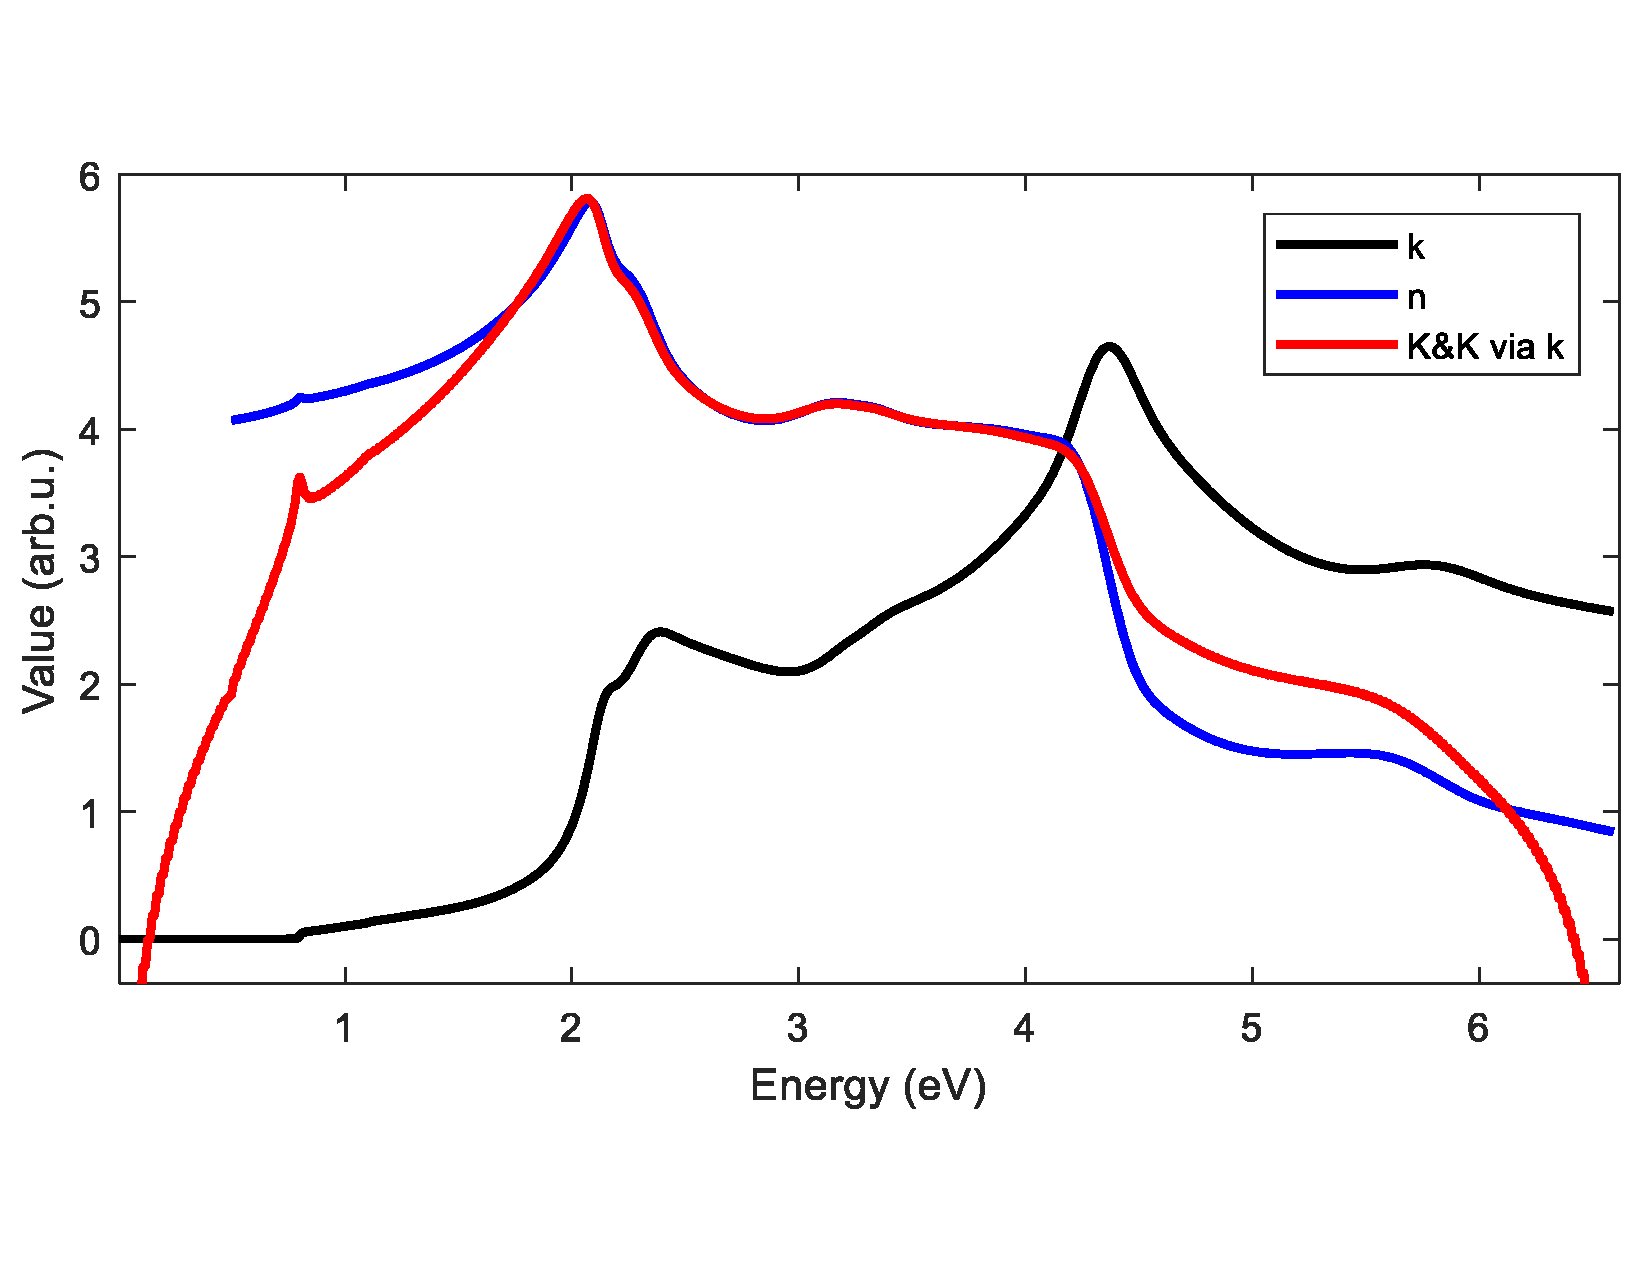
\includegraphics[width = 12cm]{Bilder/Grundlagen/KramersKronig.pdf}
    \caption{The data for the refractive index $n$ and the optical extinction parameter $\kappa$ from \cite{Nunley.2016} and the calculation of $\kappa$ using the Kramers-Kronig relations show great overlap.} 
\end{figure}

Normal and abnormal dispersion are two patterns in the refractive index. The refractive index is dependent on the
wavelength of the light. With normal dispersion, the refractive index $n$ decreases for longer wavelengths as shown in Figure \ref{fig:nglass}. This implies that photons 
with higher energy travel slower in the medium. This shape is called "normal" because it is the early on observed 
change of $n$ for glasses in the optical spectrum. For the case of abnormal dispersion $n$ increases
for growing wavelength.

\begin{figure}[ht]
    \centering
    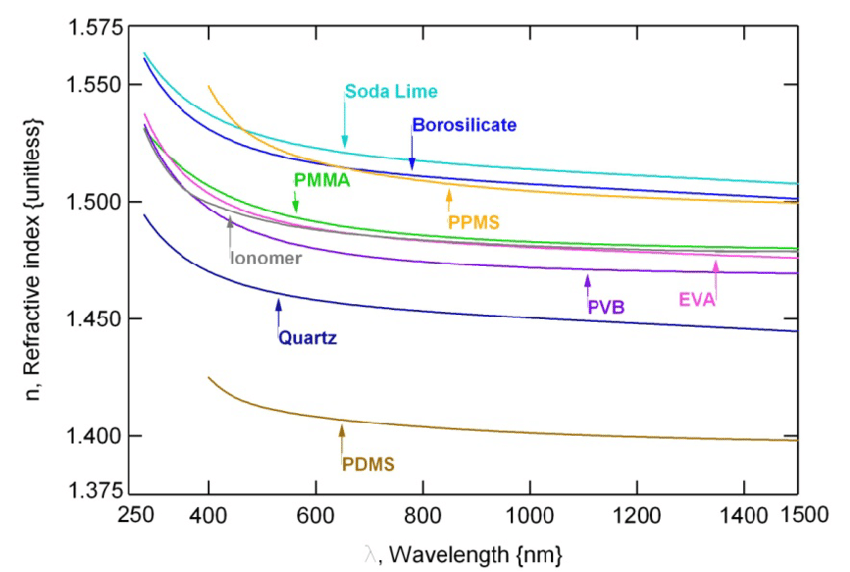
\includegraphics[width = 10cm]{Bilder/Grundlagen/DispersionGlass.png}
    \caption{Real refractive index $n$, measured or from trendline fit for candidate CPV optical materials over the wavelength range commonly utilized in PV applications. The result for FP-PV (solarized soda lime glass) is provided for reference. From \cite{Miller.2009}}
    \label{fig:nglass}
\end{figure}